%------------------------------------------------------------------------------
% Template file for the submission of papers to IUCr journals in LaTeX2e
% using the iucr document class
% Copyright 1999-2013 International Union of Crystallography
% Version 1.6 (28 March 2013)
%------------------------------------------------------------------------------

\documentclass[preprint]{iucr}              % DO NOT DELETE THIS LINE
%\documentclass[]{iucr}              % DO NOT DELETE THIS LINE
\usepackage{amssymb}
\usepackage{bm}
\usepackage[fleqn]{amsmath}
\DeclareGraphicsRule{.tif}{png}{.png}{`convert #1 `basename #1 .tif`.png}
%\usepackage{amsbsy}
\usepackage{float}
\usepackage{url}
%\usepackage{yfonts}
\usepackage{graphicx}
\usepackage{xcolor}
\usepackage[outdir=./]{epstopdf}
\usepackage{epsfig}
\usepackage{booktabs}

\newcommand{\SVI}[0]{$\bf{S^{6}}$}
\newcommand{\GVI}[0]{$\bf{G^{6}}$}
\newcommand{\scalarsub}[2]{$#1_#2$}
\newcommand{\vdotv}[2]{${{\bf #1 \cdot #2}}$}

     %-------------------------------------------------------------------------
     % Information about journal to which submitted
     %-------------------------------------------------------------------------
     \journalcode{A}              % Indicate the journal to which submitted
                                  %   A - Acta Crystallographica Section A
                                  %   B - Acta Crystallographica Section B
                                  %   C - Acta Crystallographica Section C
                                  %   D - Acta Crystallographica Section D
                                  %   E - Acta Crystallographica Section E
                                  %   F - Acta Crystallographica Section F
                                  %   J - Journal of Applied Crystallography
                                  %   M - IUCrJ
                                  %   S - Journal of Synchrotron Radiation

\begin{document}                  % DO NOT DELETE THIS LINE


     %-------------------------------------------------------------------------
     % The introductory (header) part of the paper
     %-------------------------------------------------------------------------

     % The title of the paper. Use \shorttitle to indicate an abbreviated title
     % for use in running heads (you will need to uncomment it).

	{\LARGE \emph{\today}} \\
\title{SELLA - A Program for Determining Bravais Lattice Types}
%\shorttitle{SELLA  Determining Bravais Lattice Types}

     % Authors' names and addresses. Use \cauthor for the main (contact) author.
     % Use \author for all other authors. Use \aff for authors' affiliations.
     % Use lower-case letters in square brackets to link authors to their
     % affiliations; if there is only one affiliation address, remove the [a].

\cauthor[a]{Lawrence C.}{Andrews}{larry6640995@gmail.com}{}
\author[b]{Herbert J.}{Bernstein}
\author[c]{Nicholas K.}{Sauter}

% ORCID for LCA - 0000-0002-4451-1641

\aff[a]{Ronin Institute, 9515 NE 137th St, Kirkland, WA, 98034-1820 \country{USA}}
\aff[b]{Ronin Institute, c/o NSLS-II, Brookhaven National Laboratory, Upton, NY, 11973 \country{USA}, Rochester Institute of Technology, c/o NSLS-II, Brookhaven National Laboratory, Upton, NY, 11973 \country{USA}}
\aff[c]{Lawrence Berkeley National Laboratory, 1 Cyclotron Rd., Berkeley, CA, 94720 \country{USA}}

% Use \shortauthor to indicate an abbreviated author list for use in
% running heads (you will need to uncomment it).

\shortauthor{Andrews, Bernstein, and Sauter}

     % Use \vita if required to give biographical details (for authors of
     % invited review papers only). Uncomment it.

	% lca IUCr id IUCr6401
%\vita{Author's biography}

     % Keywords (required for Journal of Synchrotron Radiation only)
     % Use the \keyword macro for each word or phrase, e.g. 
     % \keyword{X-ray diffraction}\keyword{muscle}

%\keyword{keyword}
\keyword{Unit cell reduction}
\keyword{Delaunay}
\keyword{Delone}
\keyword{Niggli}
\keyword{Selling}
\keyword{Bravais Lattice}

     % PDB and NDB reference codes for structures referenced in the article and
     % deposited with the Protein Data Bank and Nucleic Acids Database (Acta
     % Crystallographica Section D). Repeat for each separate structure e.g
     % \PDBref[dethiobiotin synthetase]{1byi} \NDBref[d(G$_4$CGC$_4$)]{ad0002}

%\PDBref[optional name]{refcode}
%\NDBref[optional name]{refcode}

\maketitle                        % DO NOT DELETE THIS LINE

\begin{synopsis}
A method for determining likely Bravais lattice types based on Selling (Delone) 
reduction. It is a complete, closed solution.
\end{synopsis}

\begin{abstract}
We introduce a new Bravais lattice determination algorithm. SELLA is a 
straight-forward algorithm and a program for determining Bravais lattice type 
based on Selling (Delone) reduction. It is a complete, closed solution, 
and it provides a clear metric of fit to each type.
\end{abstract}
		
{\bf Note:}  Boris Delaunay in his later publications used the Russian version 
of his surname: Delone. We will follow that choice.\\


     %-------------------------------------------------------------------------
     % The main body of the paper
     %-------------------------------------------------------------------------
     % Now enter the text of the document in multiple \section's, \subsection's
     % and \subsubsection's as required.

\section{Introduction}

We introduce a new Bravais lattice determination algorithm. The Bravais 
lattice types were created by \citeasnoun{Bravais1850}. \citeasnoun{Delaunay1932} 
and \citeasnoun{Niggli1928} developed methods for the identification 
of the Bravais lattice type of a crystal using the measured unit cell 
dimensions; their methods were exact only if the cell parameters 
exactly corresponded to the actual type \cite{Patterson1957}. 
Delone discussed the issues of scalars that have nearly zero values, 
but the broader issues of other measurement errors were not 
discussed. \citeasnoun{andrews2014} review the literature on 
the efforts to create methods to utilize data that contain unavoidable 
measurement error.

SELLA is a algorithm and program for determining Bravais lattice 
type based on Selling (Delone) reduction. It is a complete, closed solution, and it provides a clear metric of fit to each type.

\section{Terminology}

\citeasnoun{Delaunay1932} found that the 14 Bravais lattice types 
could be allocated among 24 types that are determined by the 
type of Dirichlet unit cell (termed the Voronoi region \cite{Voronoi1908} or 
Dirichlet region \cite{dirichlet1850} by 
Delone). Delone used the convention of \citeasnoun{Bravais1850}
with the sides of the tetrahedron labeled by the labels of the six
Selling scalars. Figure \ref{fig:PQRSTU} shows the labeling used in
the International Tables for Crystallography \cite{Henry1952}; 
Table \ref{table:ScalarConcordance} shows other choices that have been used. The
 contents for each type are described in Figure \ref{fig:terminology}.

CHARACTER

\citeasnoun{Burzlaff1985} revised the labeling of the types.
Here we have returned to the numbering of the types to that 
of \citeasnoun{Delaunay1932}.
In some cases, Delone included two forms within a single 
type. \citeasnoun{Burzlaff1985}
renumbered by ordinals. Here we have labeled the Delone 
types that have multiple items as "A" and "B". Table \ref{table:DeloneTypeConcordance}
shows the various labelings. Figure \ref{fig:DeloneTypes} 
recapitulates the figure of \citeasnoun{Delaunay1932} using 
more modern notation. Table \ref{table:ScalarConcordance} 
lists the various labelings that have been 
used for the sides of the Bravais tetrahedron. 
Figure \ref{fig:basictriangle} shows the arrangement of the 
symbols as used in the International Tables for Crystallography.

\begin{table}
		\begin{tabular}{cccccccccccc} 
			\toprule
			
	\rotatebox{80}{\citeasnoun{Delaunay1932}}
		  & \rotatebox{80}{\citeasnoun{Henry1952}  }
		   & \rotatebox{80}{\citeasnoun{Patterson1957} }
		 & \rotatebox{80}{\citeasnoun{Burzlaff1985}}
		   &\rotatebox{80}{\citeasnoun{andrews2019} } \\	
			\midrule
		g&p&P&h$_{23}$&\scalarsub{s}{1}\\		
		k&r&R&h$_{12}$&\scalarsub{s}{3}\\		
		l&s&S&h$_{14}$&\scalarsub{s}{4}\\		
		m&t&T&h$_{24}$&\scalarsub{s}{5}\\		
		h&q&Q&h$_{13}$&\scalarsub{s}{2}\\		
		n&u&U&h$_{34}$&\scalarsub{s}{6}\\		
		\bottomrule
	\end{tabular}

	\caption{The various terms used to describe the sides of 
		the Bravais tetrahedron. (In the figures in \citeasnoun{Delaunay1932} 
		the tetrahedron has been rotated by -120 degrees)}
	\label{table:ScalarConcordance}
\end{table}


\begin{table}
	\begin{tabular}{ccccccccc}
		\toprule
		 \cite{Delaunay1932} & \cite{Burzlaff1985}   &this  \\
		&  & paper \\
		\midrule
		K$_I$ & K1 & C1 \\		
		K$_{III}$ & K2 & C3 \\		
		K$_V$ & K3 & C5 \\		
		Q$_I$ & Q1 & T1 \\		
		Q$_{II}$ & Q2 & T2 \\		
		Q$_V$ & Q3 & T5\\		
		R$_I$ & R1 & R1 \\		
		R$_{III}$ & R2 & R3 \\		
		O$_I$ & O1 & O1A  \\		
		O$_I$ & O2 & O1B  \\		
		O$_{II}$ & O3 & O2   \\		
		O$_{III}$ & O4 & O3   \\		
		O$_{IV}$ & O5 & O4   \\		
		O$_V$ & O6 & O5   \\		
		M$_I$ & M1 & M1A  \\		
		M$_I$ & M2 & M1B  \\		
		M$_{II_2}$  & M3 & M2A  \\		
		M$_{II}$ & M4 & M2B  \\		
		M$_{III}$ & M5 & M3  \\		
		M$_{IV}$ & M6 & M4  \\		
		T$_I$ & T1 & A1  \\ 		
		T$_{II}$ & T2 & A2 \\		
		T$_{III}$ & T3 & A3 \\		
		H$_{IV}$  & H1 & H4 \\ 
		\bottomrule
	\end{tabular}
~\\ ~\\
	\caption{The 24 Delone types. \cite{Delaunay1932}}
	\label{table:DeloneTypeConcordance}
\end{table}

\subsection{The space \SVI{}}
\cite{andrews2019} recast the Selling parameters to define a metric space, \SVI{}.
We use the base vectors, $\bf{a}$, $\bf{b}$, $\bf{c}$ of the unit cell to define $\bf{d}=-(\bf{a}+\bf{b}+\bf{c})$.
A point ${s}$ in \SVI{} is defined as:\\
${s}$= [\scalarsub{s}{1}, \scalarsub{s}{2}, \scalarsub{s}{3},\scalarsub{s}{4}, \scalarsub{s}{5}, \scalarsub{s}{6}] \\
where \scalarsub{s}{1}=\vdotv{b}{c}, ~\scalarsub{s}{2}=\vdotv{a}{c}, ~\scalarsub{s}{3}=\vdotv{a}{b}, 
~\scalarsub{s}{4}=\vdotv{a}{d}, ~\scalarsub{s}{5}= \vdotv{b}{d}, and \scalarsub{s}{6}=\vdotv{c}{d}.

\subsection{Terminology of the Bravais lattice types}
The Bravais tetrahedron symbol. Figure \ref{fig:PQRSTU}  and Table \ref{table:DeloneTypeConcordance}\\
The different ways that the scalars have been labeled  Figure \ref{fig:terminology} \\
The table of the Delone types. Figure \ref{fig:DeloneTypes} \\


\section{Algorithms for creation of an exhaustive list of the polytopes of the Bravais types}

\subsection{Deriving the projectors and perps}

We will use Selling reduction; Niggli reduction has a fundamental 
unit that is non-convex, and some boundaries of the fundamental 
unit are partly closed and partly open \cite{andrews2014} leading 
to considerable complexity. Because Niggli reduction divides the 
fundamental unit into separate all obtuse and all acute regions, 
 the transitions between those are quite complex \cite{andrews2014}. 
In space $\bf{S^{6}}$ \cite{andrews2019b}, the fundamental 
unit is the simple all-negative orthant of a 6-dimensional 
Cartesian space. Only two kinds of operations in the space 
will need to be considered: the 6 boundary transform operations 
at the boundaries of the orthant (zeros of an axis), and 
24 reflections \cite{andrews2019}

Twenty-four lattice types were enumerated by \citeasnoun{Delaunay1932}. 
Three of those are triclinic, and we will ignore them because all crystals 
can be indexed as triclinic. We 
shall need all representations of all non-triclinic lattice 
types within the $\bf{S^{6}}$ fundamental unit (all Selling-reduced 
cells) or those generated beyond the boundaries by boundary transforms. 
Three forms (M3, M2B, and O3) are reduced dimension boundaries that do
not correspond to unique Bravais types; any lattice that falls in those
three is indexed by one of the other types.




 Seven of the 21 Delone types do not have a zero in their $\bf{S^{6}}$ 
 representation; the presence of zero indicates that a form is 
 on the boundary of the $\bf{S^{6}}$ fundamental unit. Since a 
 point on the boundary transforms to another boundary 
 point \cite{andrews2019b}, we can generate the Virtual 
 Cartesian Point (VCP) \cite{andrews2019b} appropriate to 
 each zero in the $\bf{S^{6}}$ vector. Because the reduction
  operations do not commute, in the cases where there is more 
  than one zero in the vector, all orderings of applying 
  reductions to all of the zeros must be generated. (For example, 
  for two zeros, there will be six vectors produced.) Again, 
  there may be many duplicate results. 
 
 Finally, the projectors must be computed for each of the many 
 sample vectors of the 21 types. We will also need the 
 ``perps'', the operators that give the normal vector to each 
 such manifold. For a particular polytope, the projector applied to the probe gives
 the least-squares best fit point within that polytope. Perps are computed by subtracting the 
 corresponding projector from the unit matrix. The norm of a perp times
 a probe is the distance from that polytope.
 
 \subsubsection{Generating sample vectors from all Bravais types}
 
 Step 1: Generate any random vector that contains no zero 
 values and no duplicate values.  For a later operation, 
 it should only contain values large enough that adding or
 subtracting the smallest
 representable floating point number will not change the 
 value in computer arithmetic ($DBL\_MIN$ in the C language).
 
 Step 2; For each Delone type, multiply its projector by 
 the vector from Step 1. Store  the results in a list 
 with entries for each type (see Table \ref{table:DeloneTypes} 
 for the projectors).
 
 Step 3:
 
a) If the vector contains no zeros, generate the 24 reflections
 and store in the list by type. 

\textit{\textbf{LCA--need to normalize the vectors, just like in lattice matching. ? Can we use the 
lattice matching code here?}}




b) If the vector contains one zero, apply the boundary transform operation for that boundary
to the vector, and
 store the products of the vector and its 24 reflections in the list. Note, 
 this is where the choice of $DBL\_MIN$ has effect; adding or
 subtracting such a small value will not change
 any value but zero.
 
 c) If the vector contains more than one zero and \underline{not} $DBL\_MIN$, 
 first set the zero to $DBL\_MIN$,  and then return it to 
 step b). Then set the second zero to $DBL\_MIN$ (with the
 first zero still zero), and send that result to step b). 
 If there is a third zero,  process it the same way as two zeros and return to c).
 
 Continue those steps until all the types have been processed. 
 There will be duplicates within each type,
 which will be eliminated later.
 
 
 \subsubsection{Generate projectors from sample vectors}
 
 Each vector in the list from the previous steps is a representative of one
 of the Delone types. Although a vector is a one-dimensional polytope,
 these vectors encode the information about the full polytopes of the
 Delone types in their zeros and their duplicate values.
 
 We begin by defining a function: \\ \relax
\underline{Fraction} computes the reciprocal of the 
number of elements that equal \\ \relax
 an input value or zero if there are no duplicates.
 
 The following steps will be repeated for each of the vectors in the
 list generated above. We generate a matrix \textit{m}.
 
 Step 1: Zero any elements that have been set to $DBL\_MIN$.
 
 Step 2: For each of the six scalars
 
 For i in 1-6
 	\textit{m}[i,i] = \{if \textit{Fraction}(s[i]) == 0.0 or abs(s[i]) == 0.0\} then 0.0 else \textit{Fraction}(s[i])
 	
For i in 1-6
For j in 1-6
\textit{m}[i,j] 	= \{if s[i]==s[j] or abs(s[j]) $>$ 0\} then~\textit{Fraction}(s[j]) else 0.0

Add m to a list of the projectors.

 
To finish, the duplicate projectors are removed within each type, 
leaving 239 non-triclinic projectors. (If the triclinic cases are 
included, there are 10 more.) See Table \ref{table:TypeCounts}.

 
\subsection {Measuring the fit}
The distance from the given polytope is just
the norm of the perp for that polytope applied to the probe.

\section{Degenerate Delone types}

Three of the 21 non-triclinic Delone types are only boundaries of other types. In Figure 
\ref{fig:degenerate}, Delone types M2B and M3 are in the row for orthorhombic, and
O3 is in the row for rhombohedral and tetragonal. These types do not need to
be searched for in general surveys.

\section{Verification}

\subsection{Rationale}

Most of the proposals for Bravais lattice determination in the 
presence of experimental error do not have a clear proof that 
they are complete. For many years there were verbal complaints 
that available programs would not infrequently miss experimental 
cases (for example, TRACER \cite{lawton1965} and many anecdotal 
communications).  To our knowledge, only the method of 
\cite{tomiyasu2012} has clearly demonstrated completeness. 
The justification that Sella is complete has three parts.

First: We require that the cell being tested be reduced, and
all Bravais lattice types within the \SVI{} fundamental unit (all
\SVI{} scalars negative) be generated. Therefore,
 the 24 possible forms of a 
reduced cell will be close to one of the 24 copies of the types. 
For the reflections, we do not need to consider the case of 
points near a boundary that might be outside; the boundary 
transforms must be treated for that.

Second: In the case of the boundary transform operations, we take the case of a point that is infinitesimally distant from the polytope of a 
Bravais lattice type that has one zero in its scalars. Take 
the point in the polytope that is closest to the experimental 
point. We transform both by the corresponding boundary transform 
operation. We have generated a new pair of points in a 
different location, one of which is in some representation of 
the same Bravais lattice type. The points are still 
infinitesimally distant from each other.

Third: Assume we have a point that is outside the fundamental 
unit and is near an undiscovered polytope for a Bravais lattice 
type. If the point is near a boundary defined by a single 
zero, then we apply a boundary transform to the point and to 
the Bravais polytope, bringing them both into the fundamental 
unit. If all of the variations of all of the Bravais 
lattice types within and on the fundamental unit have 
been generated, then this putative undiscovered polytope 
has already been included in the list of possibilities. 
Similar arguments apply to the cases of two or three zeros.

If we apply all of the boundary transform operations to the 
representations of the Bravais lattice types, then 
there are no places that a point in the fundamental 
unit will fail to find the closest Bravais lattice 
(or lattices). As stated above, there are 239 
non-triclinic possible representations.

What might occur if some reduced point has an unreduced 
copy near the all-negative orthant?  Would it be 
possible for it to be close to one of the copies of one 
of the 21 Delone types? The reduced point is obviously in 
the all-negative orthant. Further, because all possible 
copies of all of the Delone type manifolds have been 
generated, the reduced point will be near a copy of the 
manifold it was near when it was unreduced.

\subsection{Testing against known cells}

89539 unit cells were extracted from the Protein Data Bank 
(\citeasnoun{bernstein1977} and \citeasnoun{berman2000}). 
When evaluated with Sella, all but 57 were found at zero 
distance from the described crystal class. The 57 were 
identified as incorrect unit cells for the assigned 
crystal class; however, the distances from the assigned 
classes were small because the deviations from the 
appropriate parameters were modest (see Table \ref{tab:PDBCells}).
\begin{table}
	\label{tab:PDBCells}
	
\begin{tabular}{ccccccc}
	\toprule
PDB ID & Sp.Gr. & Delone type&distance ({{\AA}}) \\ 
\midrule
		1NUI&P3121&H4&0.0439\\ 
		2NW8&P3121&H4&0.0401\\ 
		2J1L&P3121&H4&0.0307\\ 
		1VYI&P3121&H4&0.2504\\ 
		3FZ8&P32&H4&0.0575\\ 
		2J5W&P3221&H4&0.0543\\ 
		2VAM&P3221&H4&0.1166\\ 
		1Y8J&P3221&H4&0.0389\\ 
		1F4V&P3221&H4&0.0276\\ 
		2ZP9&P6&H4&0.0528\\ 
		1DDR&P61&H4&0.0726\\ 
		1DDS&P61&H4&0.0726\\ 
		1SGU&P61&H4&0.0295\\ 
		3CDC&P61&H4&0.0559\\ 
		2WAG&P6122&H4&0.0377\\ 
		1LBM&P6122&H4&0.0312\\ 
		2O9Z&P62&H4&0.0402\\ 
		1ELZ&P6322&H4&0.4035\\ 
		1SA0&P65&H4&0.0681\\ 
		3KQI&P6522&H4&0.0331\\ 
		2F9Y&P6522&H4&0.0470\\ 
		3E73&P6522&H4&0.0523\\ 
		3CAP&H3&H4&0.0586\\ 
		2UX6&H32&H4&0.0386\\ 
		1ODT&H32&H4&0.0816\\ 
		2FDI&P43&T5&0.0758\\ 
		3HQ7&P43212&T5&0.2869\\ 
		1E2Q&P43212&T5&0.5482\\ \\
\bottomrule
\end{tabular}
\begin{tabular}{ccccccc}
	\toprule
	PDB ID & Sp.Gr. & Delone type&distance ({{\AA}}) \\ 
	\midrule
			1SHN&P43212&T5&0.0491\\ 
			1C50&P43212&T5&1.9040\\ 
			2A1L&P43212&T5&0.0528\\ 
			1S2L&P43212&T5&0.0334\\ 
			1H9S&P41&T5&1.0149\\ 
			1H9R&P41&T5&1.0141\\ 
			2F0Q&P41&T5&0.0260\\ 
			3EYM&P41&T5&0.0476\\ 
			1WV5&P41212&T5&0.0250\\ 
			2DF3&P41212&T5&0.0387\\ 
			1L6O&P41212&T5&0.0346\\ 
			3A58&P41212&T5&0.2976\\ 
			2IU9&P41212&T5&0.0373\\ 
			4BTP&P41212&T5&0.0666\\ 
			1W54&P4212&T5&0.0420\\ 
			2PBE&P42212&T5&0.0548\\ 
			3BR5&P42212&T5&0.2203\\ 
			1GMD&P42212&T5&0.1400\\ 
			1GMC&P42212&T5&0.1402\\ 
			2CCN&P42212&T5&0.0447\\ 
			1CE1&P212121&O5&0.6472\\ 
			3DQ2&P212121&O5&0.1058\\ 
			1Z2A&P212121&O5&0.0670\\ 
			2HA3&P212121&O5&0.3070\\ 
			3BNJ&I4122&T2&0.9518\\ 
			4MGP&I-42d&T1&0.2128\\ 
			4ASL&C2221&O4&0.3383\\ 
			3K7M&P432&C5&0.0517\\ 
			3GBN&I213&C1&1.2661\\ 
	\bottomrule
\end{tabular}

	\caption{}
\end{table}
\subsection{Testing for continuity}

The polytopes of the Bravais lattice types are characterized by required zeros
of scalars and/or multiplets of equal values. For instance, all primitive 
monoclinic cells have two 90 degree angles and so two zero scalars. Consider R1 as
an example for multiplets. The character for R1 is $ \bf{rrr sss} $; two triplets.

For the case of M4, primitive monoclinic, the character is $ \bf{00r stu} $. 
For a particular value for r,s,t,u, the best monoclinic cell will not
depend on whatever values are substituted for the zeros. In the plane
corresponding to the two zero scalars, we can draw a circle, each point
on the circle corresponding to a lattice. Reducing each lattice and calculating
the distance of the reduced cell from $ \bf{00r stu} $ will give a curve that
should not have any discontinuities. See Figure \ref{fig:M4}. 

Similarly, Bravais type O5 has a triplet of zeros, character $ \bf{000 rst} $. Here we
can generate a sphere that surrounds the orthorhombic point. See Figure \ref{fig:O5}.

Bravais type O4 has two zeros and a pair of required equal values, 
character $ \bf{00r sst} $. The zeros can be treated the same as above. 
The pair of equal values must 
have an average value that remains equal to $\bf{s}$ in the lattice character. 
That leaves 3 values to vary, and we can create a sphere around 
the point $ \bf{00r sst} $. See Figure \ref{fig:O4}.



\section{Comparisons}

Comparison to other distance measure; Data for other measures taken
from \citeasnoun{andrews2014}.

\begin{tabular}{ccccccc}
	\toprule
	Lattice character&G6 distance  &BGAOL   Z score&XDS QI &Scaled QI &Sella\\	
	\midrule
			mP               &     20.138  & 0.657    &   1.0  & 0.13  & 1.06\\	
			oC               &     125.958 &  3.560   &    23. & 8 3.09& 13.82\\	
			mC               &     125.150 &  4.085   &    23. & 4 3.03& 13.80\\	
	\bottomrule
\end{tabular}

~\\



     % Appendices appear after the main body of the text. They are prefixed by
     % a single \appendix declaration, and are then structured just like the
     % body text.

     %-------------------------------------------------------------------------
     % The back matter of the paper - acknowledgements and references
     %-------------------------------------------------------------------------

     % Acknowledgements come after the appendices
     
     
	\ack{{\bf Acknowledgements}}
	Careful copy-editing and corrections by Frances C. Bernstein are 
gratefully acknowledged.  	Our thanks to Jean Jakoncic and Alexei Soares for 
helpful conversations and access to data and facilties at 
Brookhaven National Laboratory.
     % References are at the end of the document, between \begin{references}
     % and \end{references} tags. Each reference is in a \reference entry.

	\ack{{\bf Funding information}}      

Funding for this research was provided in part by: US Department of Energy Offices of Biological and Environmental Research and of Basic Energy Sciences (grant No. DE-AC02-98CH10886 ; grant No. E-SC0012704); U.S. National Institutes of Health (grant No. P41RR012408; grant No. P41GM103473; grant No. P41GM111244; grant No. R01GM117126, grant No. 1R21GM129570; grant No. P30GM133893); Dectris, Ltd.

\bibliographystyle{iucr}
\bibliography{Reduced}

     %-------------------------------------------------------------------------
     % TABLES AND FIGURES SHOULD BE INSERTED AFTER THE MAIN BODY OF THE TEXT
     %-------------------------------------------------------------------------

     % Simple tables should use the tabular environment according to this
     % model
     
\begin{table}
\caption{The 21 non-triclinic Delone types with the count of representations.
The asterisks indicate non-crystallographic types.}
\label{table:TypeCounts}
\begin{tabular}{lr}
Delone type & Count    \\
\hline
H4&12\\
C1&1\\
C3&3\\
C5&16\\
R1&4\\
R3&12\\
T1&3\\
T2&6\\
T5&48\\
O1A&3\\
O1B&1\\
O2&6\\
O3$^*$&9\\
O4&36\\
O5&16\\
M1A&6\\
M1B&3\\
M2A&12\\
M2B$^*$&12\\
M3$^*$&18\\
M4&12\\
\bottomrule
\end{tabular}
\end{table}
    
\fontseries{Courier}{
\begin{table}
	\caption{Projectors for the 24 Delone types}
	\label{table:DeloneTypes}
	\begin{tabular}{lcl}
		\toprule
C1  & (cI) & [1 1 1 1 1 1/  1 1 1 1 1 1/  1 1 1 1 1 1/  1 1 1 1 1 1/  1 1 1 1 1 1/  1 1 1 1 1 1] \\ 
C3  & (cF) & [1 1 0 1 1 0/  1 1 0 1 1 0/  0 0 0 0 0 0/  1 1 0 1 1 0/  1 1 0 1 1 0/  0 0 0 0 0 0] \\ 
C5  & (cP) & [0 0 0 0 0 0/  0 0 0 0 0 0/  0 0 0 0 0 0/  0 0 0 1 1 1/  0 0 0 1 1 1/  0 0 0 1 1 1] \\ \\

T1  & (tI) & [1 1 0 1 1 0/  1 1 0 1 1 0/  0 0 1 0 0 1/  1 1 0 1 1 0/  1 1 0 1 1 0/  0 0 1 0 0 1] \\ 
T2  & (tI) & [1 1 0 1 1 0/  1 1 0 1 1 0/  0 0 0 0 0 0/  1 1 0 1 1 0/  1 1 0 1 1 0/  0 0 0 0 0 1] \\ 
T5  & (tP) & [0 0 0 0 0 0/  0 0 0 0 0 0/  0 0 0 0 0 0/  0 0 0 1 1 0/  0 0 0 1 1 0/  0 0 0 0 0 1] \\ \\

R1  & (rP) & [1 1 1 0 0 0/  1 1 1 0 0 0/  1 1 1 0 0 0/  0 0 0 1 1 1/  0 0 0 1 1 1/  0 0 0 1 1 1] \\ 
R3  & (rP) & [1 1 0 0 1 0/  1 1 0 0 1 0/  0 0 0 0 0 0/  0 0 0 1 0 0/  1 1 0 0 1 0/  0 0 0 0 0 0] \\ \\

O1A & (oF) & [1 1 0 1 1 0/  1 1 0 1 1 0/  0 0 1 0 0 0/  1 1 0 1 1 0/  1 1 0 1 1 0/  0 0 0 0 0 1] \\ 
O1B & (oI) & [1 0 0 1 0 0/  0 1 0 0 1 0/  0 0 1 0 0 1/  1 0 0 1 0 0/  0 1 0 0 1 0/  0 0 1 0 0 1] \\ 
O2  & (oI) & [1 0 0 0 1 0/  0 1 0 1 0 0/  0 0 0 0 0 0/  0 1 0 1 0 0/  1 0 0 0 1 0/  0 0 0 0 0 1] \\ 
O3  & (oI) & [1 0 0 1 0 0/  0 1 0 0 1 0/  0 0 0 0 0 0/  1 0 0 1 0 0/  0 1 0 0 1 0/  0 0 0 0 0 0] \\ 
O4  & (oS) & [0 0 0 0 0 0/  0 0 0 0 0 0/  0 0 1 0 0 0/  0 0 0 1 1 0/  0 0 0 1 1 0/  0 0 0 0 0 1] \\ 
O5  & (oP) & [0 0 0 0 0 0/  0 0 0 0 0 0/  0 0 0 0 0 0/  0 0 0 1 0 0/  0 0 0 0 1 0/  0 0 0 0 0 1] \\ \\

M1A & (mC) & [1 1 0 0 0 0/  1 1 0 0 0 0/  0 0 1 0 0 0/  0 0 0 1 1 0/  0 0 0 1 1 0/  0 0 0 0 0 1] \\ 
M1B & (mC) & [1 0 0 1 0 0/  0 1 0 0 1 0/  0 0 1 0 0 0/  1 0 0 1 0 0/  0 1 0 0 1 0/  0 0 0 0 0 1] \\ 
M2A & (mC) & [1 0 0 1 0 0/  0 1 0 0 1 0/  0 0 0 0 0 0/  1 0 0 1 0 0/  0 1 0 0 1 0/  0 0 0 0 0 1] \\ 
M2B & (mC) & [1 0 0 0 0 0/  0 1 0 1 0 0/  0 0 0 0 0 0/  0 1 0 1 0 0/  0 0 0 0 1 0/  0 0 0 0 0 1] \\ 
M3  & (mC) & [1 0 0 0 0 0/  0 1 0 0 1 0/  0 0 0 0 0 0/  0 0 0 1 0 0/  0 1 0 0 1 0/  0 0 0 0 0 0] \\ 
M4  & (mP) & [0 0 0 0 0 0/  0 0 0 0 0 0/  0 0 1 0 0 0/  0 0 0 1 0 0/  0 0 0 0 1 0/  0 0 0 0 0 1] \\ \\

A1  & (aP) & [1 0 0 0 0 0/  0 1 0 0 0 0/  0 0 1 0 0 0/  0 0 0 1 0 0/  0 0 0 0 1 0/  0 0 0 0 0 1] \\ 
A2  & (aP) & [1 0 0 0 0 0/  0 1 0 0 0 0/  0 0 0 0 0 0/  0 0 0 1 0 0/  0 0 0 0 1 0/  0 0 0 0 0 1] \\ 
A3  & (aP) & [1 0 0 0 0 0/  0 1 0 0 0 0/  0 0 0 0 0 0/  0 0 0 1 0 0/  0 0 0 0 1 0/  0 0 0 0 0 0] \\ \\

H4  & (hP) & [0 0 0 0 0 0/  0 0 0 0 0 0/  0 0 1 1 1 0/  0 0 1 1 1 0/  0 0 1 1 1 0/  0 0 0 0 0 1] \\ 
\bottomrule
	\end{tabular}
\end{table}
}
     % Postscript figures can be included with multiple figure blocks


\begin{figure}
\caption{Bravais triangle with labeling as used in the International Tables}
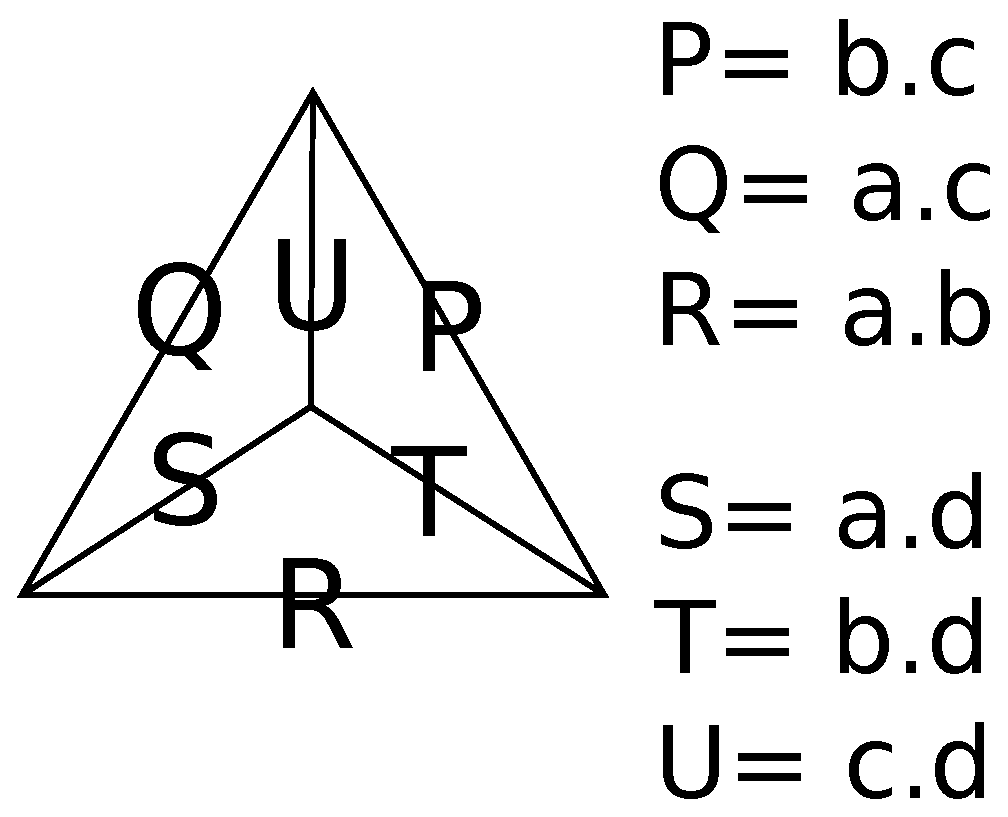
\includegraphics[width=3cm]{PQRSTU}
\label{fig:PQRSTU}
\end{figure}

\begin{figure}
	\caption{Delone type description}
	\label{fig:terminology}
	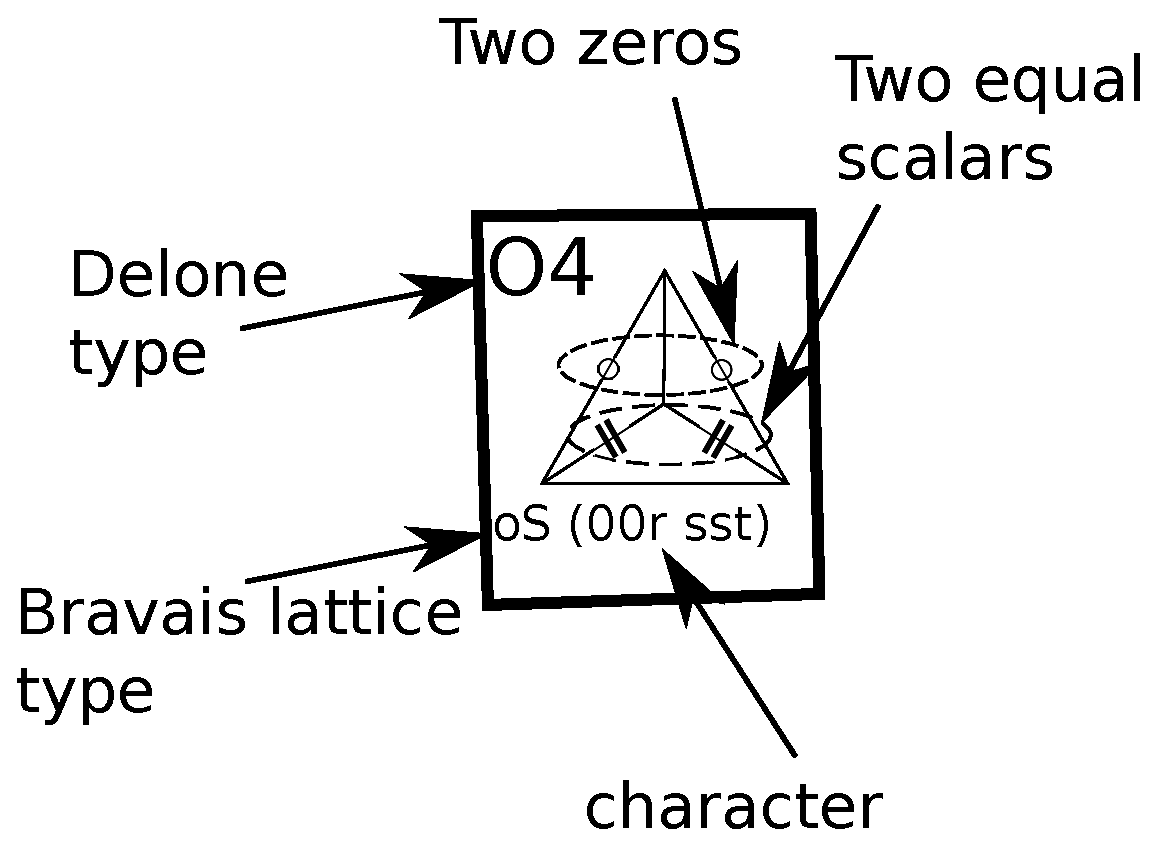
\includegraphics[width=12cm]{terminology}
\end{figure}

\begin{figure}
	\caption{The Delone types}
	\label{fig:DeloneTypes}
	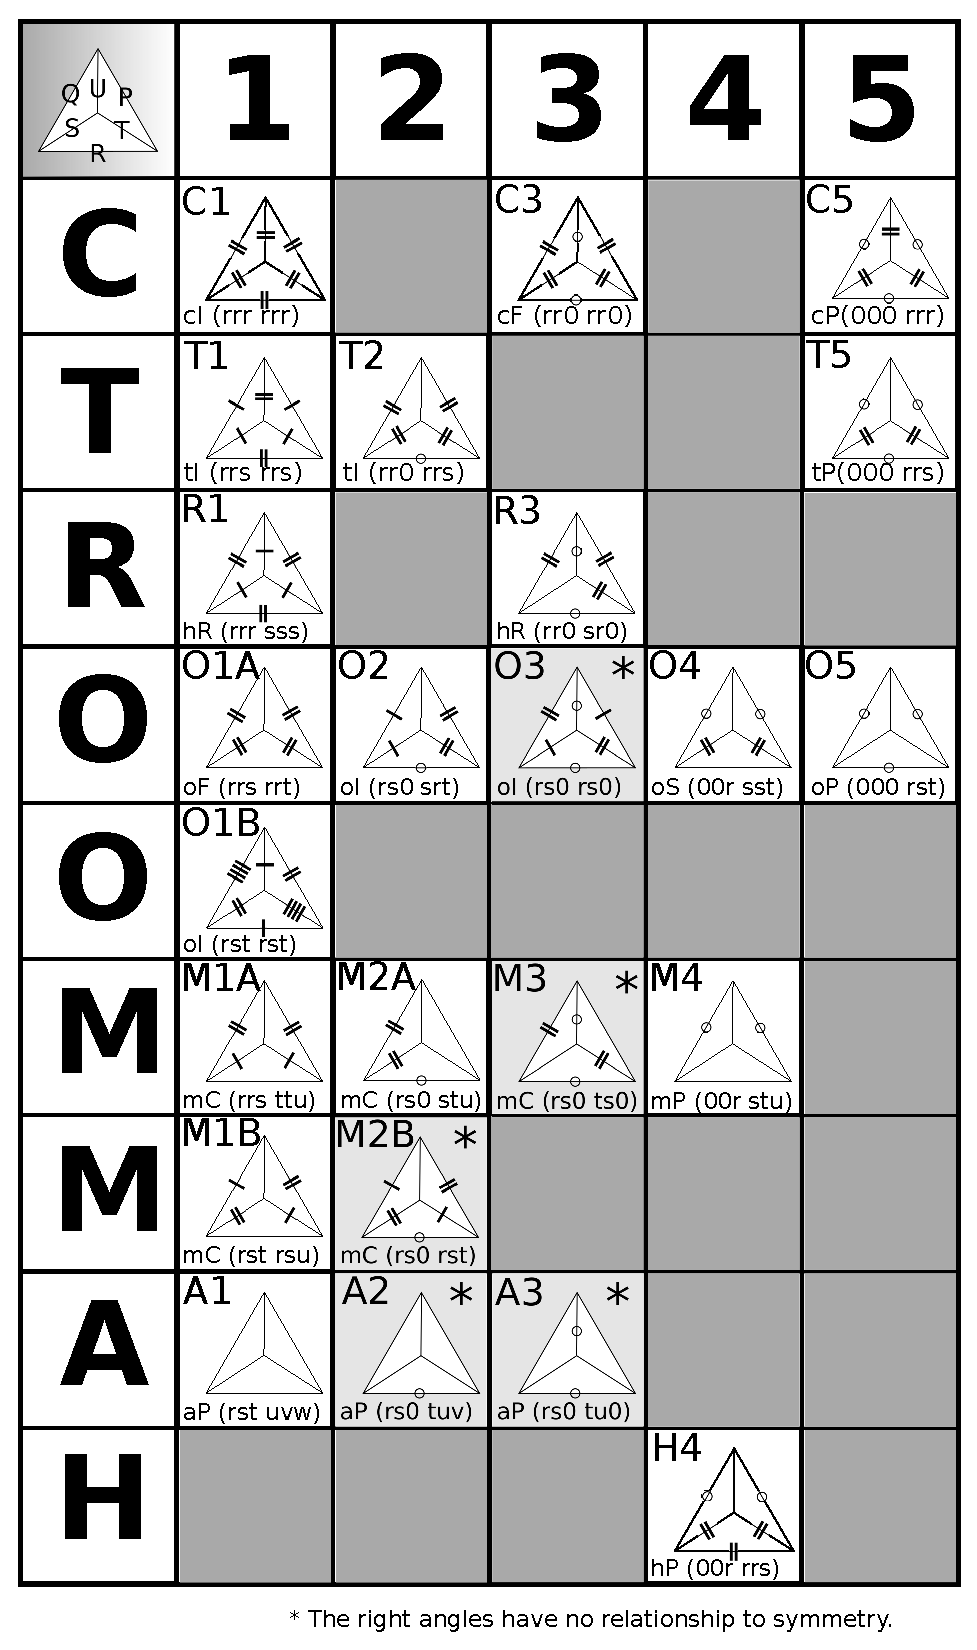
\includegraphics[width=12cm]{DeloneTypesGrid_2}
\end{figure}

\begin{figure}
	\caption{}
	\label{fig:degenerate}
	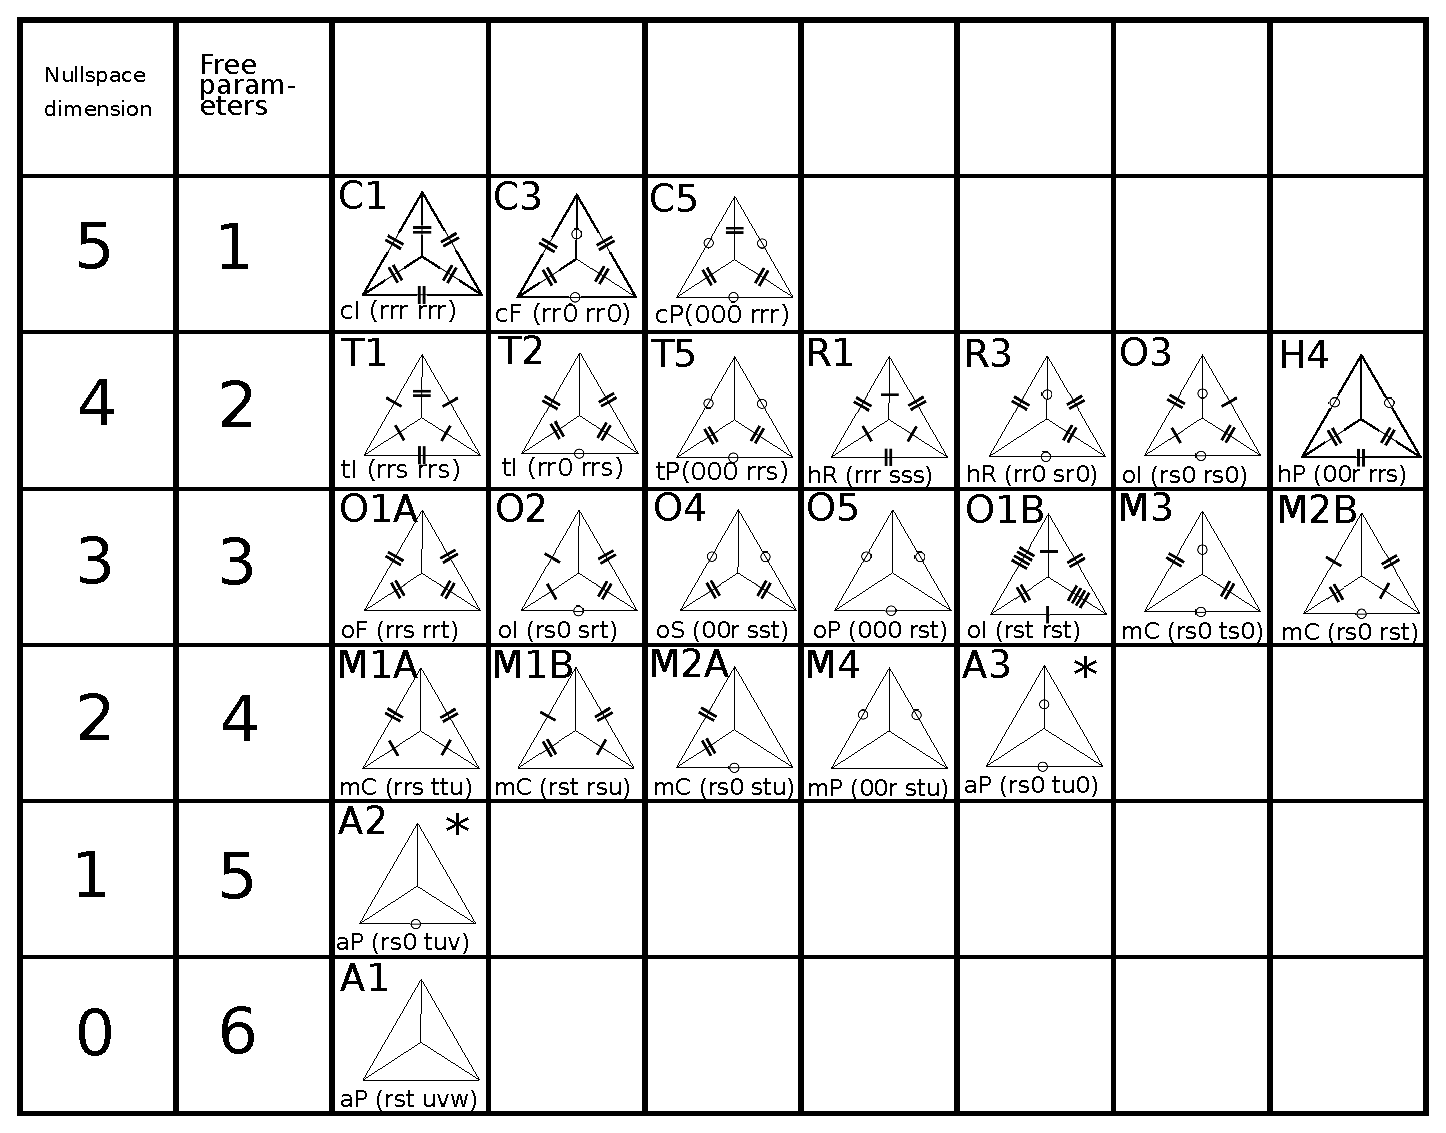
\includegraphics[width=12cm]{NullSpaceDistribution}
\end{figure}

\begin{figure}
	\label{fig:M4}
	\caption{Delone type M4: there are two zeros. A circle of 100 points with
		radius 0.1 is centered at 0,0. The lattices are reduced and the points are
		plotted at the distance from M4.} The red points indicate the original
	circle. The blue points are for the reduced cells.
	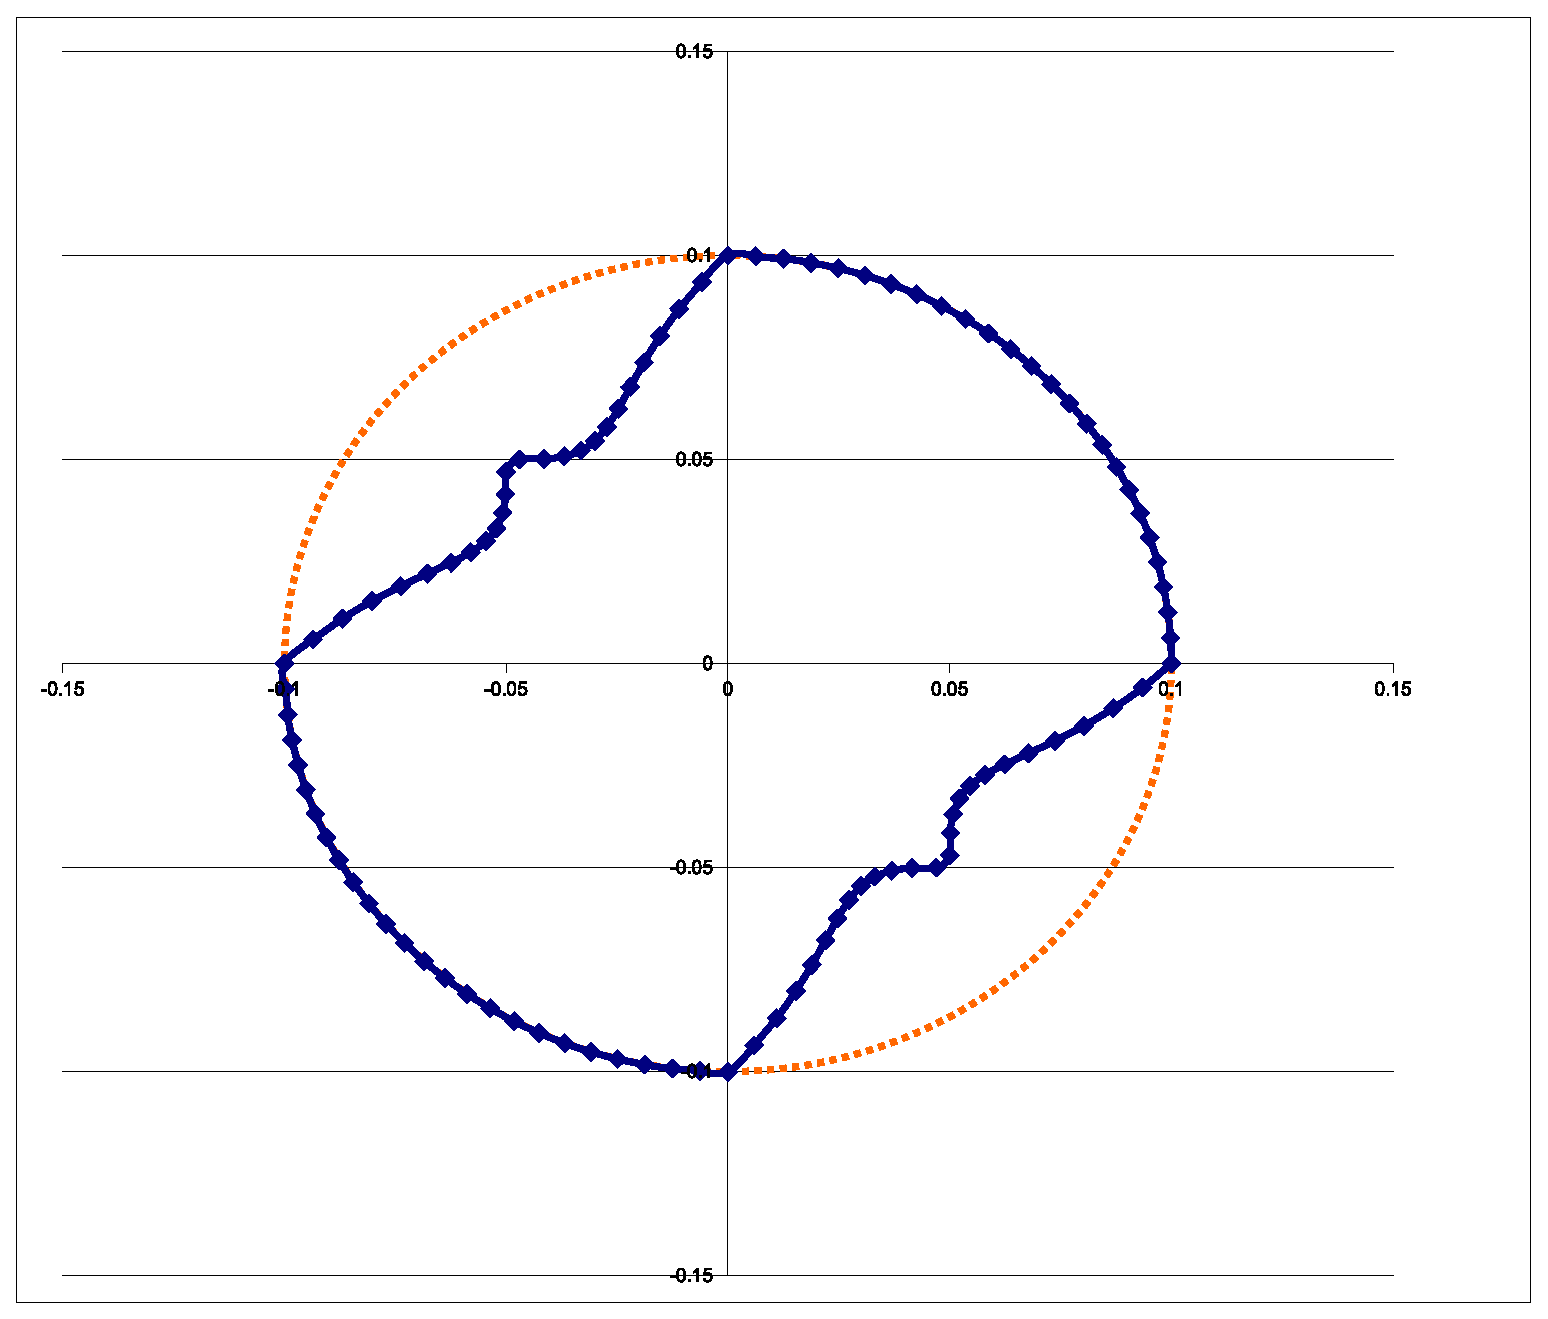
\includegraphics[width=12cm]{M4-100-2-zeros}
\end{figure}

\begin{figure}
	\caption{Delone type O5: there are three zeros. A sphere 
		is centered at 0,0,0, with radius 0.1. The lattices are 
		reduced, and the point is 
		placed at a distance equal to the distance from type O5. 50,000
		points are plotted.}
	\label{fig:O5}
	\includegraphics[width=12cm]{O5-50K-3-zeros}
\end{figure}

\begin{figure}
	\caption{Delone type O4: There are two zeros and one pair.
	A sphere with radius 0.1 was placed around one point. At each
sphere point, the lattice was reduced and the point on the sphere
was assigned a color (0.01) to blue (0.0075). 100,000 points are plotted.}
	\label{fig:O4}
	\includegraphics[width=12cm]{O4_Cropped-2-zeros-1-pair}
\end{figure}

\end{document}                    % DO NOT DELETE THIS LINE
%%%%%%%%%%%%%%%%%%%%%%%%%%%%%%%%%%%%%%%%%%%%%%%%%%%%%%%%%%%%%%%%%%%%%%%%%%%%%%
